% preambule dokumentu
\documentclass[12pt]{article}
\usepackage[utf8]{inputenc}
\usepackage[czech]{babel}
\usepackage{cite}
\usepackage[pdf]{graphviz}
\usepackage{mathtools}
\usepackage{dipp8, xltxtra, graphicx}
\usepackage{pgfplots}
\usepackage{amsfonts}
\usepackage{neuralnetwork}
\usepackage[hidelinks]{hyperref}
\usepackage{listings}
\usepackage{plantuml}
\usepackage{float}

%% Definice javascriptu
\lstdefinelanguage{JavaScript}{%
	keywords={const, let, typeof, instanceof, new, true, false, catch, function, return, null, undefined, catch, switch, var, if, in, while, for, do, else, case, break},
	keywordstyle=\bfseries,
	ndkeywords={class, export, throw, import, this},
	ndkeywordstyle=\bfseries,
	sensitive=false,
	comment=[l]{//},
	morecomment=[s]{/*}{*/},
	commentstyle=\ttfamily,
	stringstyle=\color{blue}\ttfamily,
	morestring=[b]',
	morestring=[b]`,
	morestring=[b]"
}

\begin{document}
\pagestyle{headings}

\def\typprace{Diplomová}

% uvodni cast zaverecne prace
\titul{Řízení autonomního agenta pomocí neuroevoluce}{Bc. Martin Hnátek}{Ing. Jiří Lýsek, Ph.D.}{Brno, 2018}
\podekovani{Rád bych zde poděkoval svému vedoucímu Ing. Jiří Lýskovi, Ph.D. za jeho cenné rady a čas, který mi věnoval při řešení této práce.}
\prohlasenimuz{V~Brně dne \today}

\abstract{Autonomous agent control using neuroevolution}{Thesis describe theory behind neuroevolution. Then it describes both design and creation of simulated environment for autonomous agent and its training with library Neataptic in environemnts with various difficulity. Thesis also describes process of designing frontend for visualization of results and backend for faster training of agents. At the end it describes resulting agents and proposes enhancements to existing solution.}
\\
\\
\textbf{Key words:}
\newline{}
NEAT, AI, MachineLearning, Agent, Javascript


\abstrakt{Řízení autonomního agenta pomocí neuroevoluce}{Tato práce představuje teoretický základ neuroevoluce. Zahrnuje také návrh tvorbou simulačního prostředí, pro autonomního agenta a jeho natrénování s pomocí knihovny Neataptic v různě obtížných podmínkách. Popisuje také tvorbu frontendu pro snadnou vizualizaci a serverové části pro rychlé učení. Na závěr se zabývá vyhodnocením natrénovaných agentů a návrhem možných zlepšení.}
\\
\\
\textbf{Klíčová slova:}
\newline{}
NEAT, AI, MachineLearning, Agent, Javascript
%+ Taky se v praci venujete nejakym teoretickym vychodiskum
%+ Pouzijete nejakou knihovnu pro neuroevoluci
%+ Vyhodnoceni vysledku
%+ ...
%Abstrak by mel jmenovat temer vse, cim se prace zabyva.
\obsah
\listoffigures
\newpage{}
\listoftables
\cislovat{2}

% jednotlive kapitoly dokumentu
\kapitola{Úvod a cíl práce}
\sekce{Úvod do problematiky}
S růstem výpočetního výkonu a rozvojem \textbf{GPUGPU} (paralelizace výpočtů na grafické kartě) se neuronové sítě ukázaly jako mocný nástroj pro řešení složitých problémů na které standardní metody umělé inteligence nestačily.

Další oblastí umělé inteligence, které nárust masivní paralelizace prospěl, jsou metaheuristiky, které mohou  s nárůstem výpočetního výkonu v rozmném čase pokrýt stále větší stavový prostor a jsou tedy schopné rychle řešit stále složitější problémy.


Neuroevoluce propojuje oba přístupy a využívá je ke generování topologii neuronových sítí a nastavení jejích vah. Výsledkem je neuronová síť, jejiž architektura lépe popisuje daný problém a lze jí aplikovat i na problémy na které by klasické neuronové sítě aplikovat nešly. Jedná se například o problémy, u kterých je těžké získat trénovací data a nelze tedy neuronovou síť natrénovat klasickými metodami, jako je například gradientní sestup.

\sekce{Cíl práce}
Cílem této práce je navrhnout a vytvořit simulační prostředí pro autonomního agenta. Poté na simulovaném prostředí provést serii experimentů, které slouží k zjištění limitů učících schopností algoritmu NEAT.

\sekce{Neuronové sítě}

Neuronové sítě jsou model strojového učení, který je volně založený na principu zvířecího mozku \cite[s.~41]{fundementalsOfDeepLearning}.

\sekce{Neuron}
Neuron je základní  výpočetní jednotka neuronových sítí, která je definovaná jako suma všech jejích vstupů a aplikace aktivační funkce.
	$$\sigma(\Sigma_{i=0}^{N} \theta_i \cdot x_{i} + b)$$
Kde:
\begin{enumerate}
	\item $\sigma$ - aktivační funkce
	\item $\theta$ - skrytá váha pro daný vstup
	\item b - bias neuronu
\end{enumerate}

\sekce{Vrstva}
Vrstva je skupina neuronů se stejnou aktivační funkcí. 

\podsekce{Aktivační funkce}
Aktivační funkce se používá pro definování výstupu a zavedení nelinearity. Bez nich by byla neuronová síť schopna aproximovat pouze n-dimenzionální rovinu. \cite[s.~65]{fundementalsOfDeepLearning} \\
Dalším využitím je omezení výstupních hodnot. Například aktivační funkce sigmoid se s oblibou používá u výstupní vrstvy neuronových sítí určených ke klasifikačním problémům, protože je to relace $\mathbb{R} \rightarrow \{0..1\}$, která se dá jednoduše jako "jistota" neuronu, že se jedná o výstup, který neuron reprezentuje. Podobně se dá uvažovat i o funkcích jako je například softmax a tanh, které také najdou hojné využití u klasifikačních problémů.

\podsekce{Linearní funkce}
Vrací vstup, tak jak je. Využití najde především u vstupní vrstvy neuronové sítě a u neuronových sítí, které řeší regresní typy úloh.
\\
\begin{tikzpicture}
\centering
\begin{axis}[grid=major, xlabel=$x$, ylabel={$f(x)$}]
\addplot[blue, samples=100, smooth, unbounded coords=discard]
plot (\x, \x);
\end{axis}
\end{tikzpicture}
$$f(x) = x$$
\podsekce{Sigmoid}
Sigmoid je aktivační funkce, která je schopná potlačit extrémní hodnoty 

\begin{tikzpicture}
\centering
\begin{axis}[grid=major, xlabel=$x$, ylabel={$f(x)$}]
\addplot[blue, samples=100, smooth, unbounded coords=discard]{1 / (1 + e ^ (-\x))};
\end{axis}
\end{tikzpicture}
$$f(x) = \frac{1}{1 + e^{-x}}$$
\podsekce{Tanh}

\textbf{Tanh} je funkce obdobná sigmoidu. Hlavní rozdíl mezi ní a sigmoidem je ten, že její obor je v rozmezí -1 a 1 hodí se proto i pro záporná výstupy, které vyžadují záporná čísla. \cite[s.~67]{fundementalsOfDeepLearning}

\begin{tikzpicture}
\centering
\begin{axis}[grid=major, xlabel=$x$, ylabel={$f(x)$}]
\addplot[blue, samples=100, smooth, unbounded coords=discard]{tanh(x)};
\end{axis}
\end{tikzpicture}
$$f(x) = tanh(x)$$
\podsekce{RELU}
RELU je aktivační funkce, která je podobná lineární aktivační funkci s tím rozdílem, že pokud vstupní hodnota nepřesáhne určitého prahu výstupem je 0. Její hlavní výhodou je to, že zabraňuje problémům s takzvaným explodujícím gradientem \cite[s.~69]{fundementalsOfDeepLearning} \\

\begin{tikzpicture}
\centering
\begin{axis}[grid=major, xlabel=$x$, ylabel={$f(x)$}]
\addplot[blue, samples=100, smooth, unbounded coords=discard]{max(0, x)};
\end{axis}
\end{tikzpicture}
\[ 
f(x) = 
\begin{dcases*} 
\text{$x>=0$,} & $x$ \\ 
\text{$x<0$,} & 0 
\end{dcases*} 
\]
\podsekce{Rekurentní neurony}
Speciální druh neuronů, který si dokáže zapamatovat a reagovat na sekvenci vstupů. Rekurentní neurony značně rozšiřují možnosti neuronových sítí. S nimi je možné řešit složité úlohy typu strojového překladu nebo sémantické vyhodnocování textu.

V praxi se setkáváme s dvěma druhy neuronů a to LSTM a novější GRU. LSTM a GRU jsou si velmi podobné s jedním podstatným rozdílem. U GRU bylo prokázáno, že je značně rychlejší. 


\kapitola{Genetické algoritmy}
Genetické algoritmy slouží k řízenému prohledávání stavového prostoru založené na teorii evoluce. \cite[s.~17]{kozaGP}
\sekce{Princip}
Základní myšlenka spočívá ve vygenerování náhodných jedinců (řešení problému) a jejích postupné zlepšování s pomocí operací křížení a mutace. Proces zlepšování genomů probíhá na základě jeho hodnocení (fitness).

Samotný algoritmus pak lze rozdělit na následující kroky \cite[s.~12]{geneticAlgorithms}

\begin{enumerate}
	\item Vygeneruj náhodnou populaci o n chromozomech
	\item Pro každý chromozom spočítej jeho fitness
	\item Opakuj dokud není splněná podmínka ukončení
	\begin{enumerate}
		\item Vyber pár chromozomů na základě jejích ohodnocení (selekce)
		\item Proveď spojení chromozomů (křížení)
		\item S určitou pravděpodobností mutuj daného jedince (mutace)
	\end{enumerate}
	\item Nahraď současnou populaci populací, která vznikla předchozím krokem
	\item Jdi na krok 2
\end{enumerate}

\sekce{Kódování}
Někdy se mu též říká genotyp je způsob zápisu řešení problému. Je důležité zároveň uvést pojem fenotyp který označuje vlastní řešení úlohy.

Existuje mnoho různých kódování a každý má své výhody a nevýhody. Většinou se snažíme vybírat kódování, které dobře reprezentuje daný problém. Zde je seznam několika nejpoužívanějších kódování \cite[s.~42-43]{geneticCZ}:
\begin{enumerate}
	\item Binární - řetězec bitů, který může například reprezentovat jednu nebo více numerických hodnot. 
	\item Reálná čísla - Jedno nebo více reálných čísel
	\item Kombinatorické - Může být například seznam čísel označujících 
\end{enumerate}
\sekce{Křížení}
Křížení je operátor, který kombinuje dva jedince do jednoho. Jedinec, který vzniká přebírá genetickou informaci od obou jedinců v určitém poměru. Jeho implementace je závislá na použitém kódování. 

Příkladem může být obrázek \ref{fig:crossover} ve kterém je ilustrováno tzv. jednobodové křížení \cite[s.~50]{geneticCZ} při kterém dochází k rozdělení obou genomů ve stejném bodě a spojením vzniklých podřetězců do nového genomu.
	
\begin{figure}[ht]
	\centering
	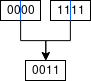
\includegraphics[scale=0.95]{crossover}
	\caption{Příklad křížení}
	\label{fig:crossover}
\end{figure}

\sekce{Mutace}
Mutace náhodně modifikuje chromozom a zavádí tak do populace variaci. Díky tomuto se může algoritmus dostat z lokálního extrému. 

Existují různé varianty mutace, která se provádí v závislosti na daném kódování. 

Například u binárního kódování se může jednat o náhodnou inverzi některého z bitů genomu viz obrázek \ref{fig:mutation}.

\begin{figure}[h!]
	\centering
	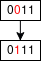
\includegraphics[scale=1.0]{mutation}
	\caption{Příklad mutace}
	\label{fig:mutation}
\end{figure}

\sekce{Selekce}
Selekce je proces výběru dvou jedinců na něž jsou později aplikovány genetické operátory jako je křížení a mutace. 

\sekce{Využití}
Genetické algoritmy naleznou využití v mnoha optimalizačních úlohách. Příkladem může být experiment, který zahrnoval použití gramatické evoluce pro vytvoření regresních modelů pro datasety CASY3 a CASY5 \cite[s.~2-9]{differentialEvolution}.

\kapitola{NEAT}
NEAT (neuroevolution of augmenting topologies) kombinuje neuronové sítě s genetickými algoritmy. Hlavní výhodou této metody je, že generuje jak topologii neuronové sítě, tak její váhy. Výsledkem může být neuronová síť jejíž rozložení lépe popisuje řešený problém.

Algoritmus probíhá stejně jako běžný genetický algoritmus. Rozdílem je použitý fenotyp a operátory mutace a křížení, které se nad ním provádí.

\sekce{Genotyp a fenotyp}
Genotyp a fenotyp je ilustrován na obrázku \ref{fig:neatgenotypetophenotype}. Genotyp obsahuje jak údaje o jednotlivých neuronech, tak informace o topologii sítě. Metadata, která se týkají topologie neuronové síti jsou údaje o spojení (IN, OUT), váha samotného spojení (weight), informace týkající se toho, zda je spojení použito v fenotypu (ENABLED/DISABLED) a inovační skore. Inovační skore je číslo, které reprezentuje pořadí ve kterém se daný gen objevil v fenotypu \cite[s.~9]{NEAT}. 

\begin{figure}[h!]
	\centering
	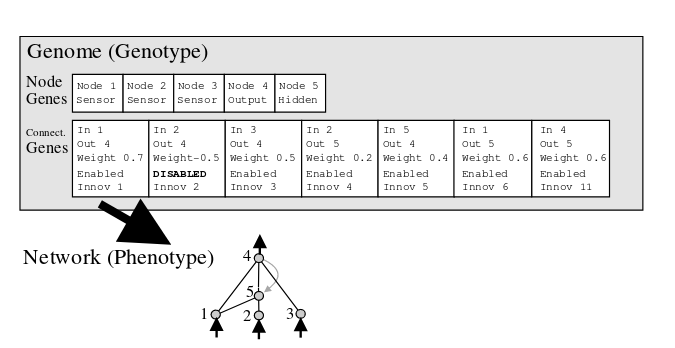
\includegraphics[width=0.7\linewidth]{neatGenotypeToPhenotype}
	\caption{Genotyp a fenotyp u algoritmu NEAT převzato z \cite[s.~9]{NEAT}}
	\label{fig:neatgenotypetophenotype}
\end{figure}

\sekce{Mutace}
Jak jíž bylo zmíněno nad fenotypem lze provádět různé operace včetně operátoru mutace, který provede náhodnou změnu fenotypu s nadějí, že změna povede k zlepšení řešení. V případě algoritmu NEAT je operátor mutace ilustrován na obrázku \ref{fig:neatmutation}. Na obrázku je vidět, že mutace může buď přidat další spojení nebo další neuron. V případě, že je přidávan nový neuron je mu přiřazeno náhodné spojení, které je označeno znakem DISABLED \cite[s.~10]{NEAT}.

\begin{figure}[h!]
	\centering
	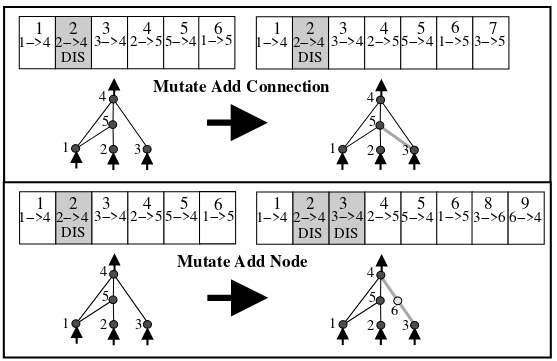
\includegraphics[scale=0.3]{neatMutation}
	\caption{Mutace v NEAT převzato z \cite[s.~10]{NEAT}}
	\label{fig:neatmutation}
\end{figure}

\sekce{Křížení}
Posledním operátorem používaným při algoritmu NEAT je operátor křížení. Operátor křížení ilustruje obrázek \ref{fig:neatcrossover}. Křížení probíhá na základě inovačního čísla. Spojení se stejným inovačním číslem jsou náhodně zděděny z rodičovských genů. Je tu také šance na převzetí genů, které vytváří spojení nenacházející se v jednom z rodičů. Tyto geny jsou převzaty pouze z rodiče, který ma větší fitness. Při křížení je také náhodná šance, která může převzatý genom vypnout \cite[s.~12]{NEAT}.

\begin{figure}[h!]
	\centering
	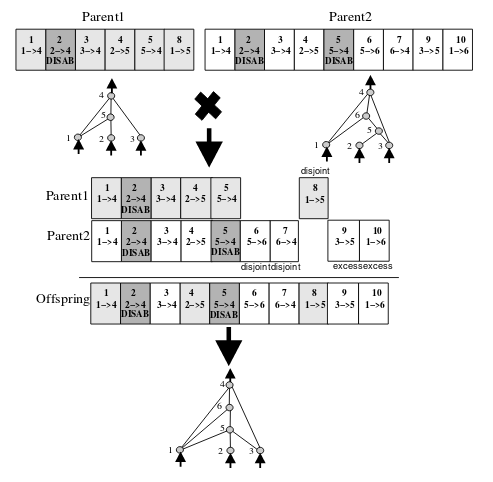
\includegraphics[width=0.6\linewidth]{neatCrossover}
	\caption{Křížení v NEAT. Převzato z \cite[s.~12]{NEAT}}
	\label{fig:neatcrossover}
\end{figure}

\sekce{Rozšíření algoritmu NEAT}
Jelikož je algoritmus NEAT v současnosti předmětem aktivního výzkumu existuje pro něj mnoho rozšíření. Tato sekce se bude zabývat některými z nich.

\podsekce{Instinct}
Instinct rozšiřuje původní algoritmus o rekurentní neurony. Rozšíření tak umožňuje případnému agentovi reagovat nejen na okamžitou situaci ale i na předchozí události ve světě. Tento fakt značně rozšiřuje možnosti neuronových sítí, které jsou generované tímto algoritmem ale zároveň je třeba mít na paměti, že se tímto značně zvětšuje prohledávaný stavový prostor a dochází tím k zvýšené časové náročnosti na získání vhodných výsledků.
\podsekce{odNEAT}
Varianta algoritmu NEAT aplikovaná na distribuované online učení skupiny autonomních robotů \cite[s.~1]{odNEAT}.
\podsekce{rtNEAT}
Rozšíření, které se zaměřuje na neuroevoluci agentů v realném čase.
%In 2003 Stanley devised an extension to NEAT that allows evolution to occur in real time rather than through the iteration of generations as used by most genetic algorithms. The basic idea is to put the population under constant evaluation with a "lifetime" timer on each individual in the population. When a network's timer expires its current fitness measure is examined to see whether it falls near the bottom of the population, and if so it is discarded and replaced by a new network bred from two high-fitness parents. A timer is set for the new network and it is placed in the population to participate in the ongoing evaluations.

%The first application of rtNEAT is a video game called Neuro-Evolving Robotic Operatives, or NERO. In the first phase of the game, individual players deploy robots in a 'sandbox' and train them to some desired tactical doctrine. Once a collection of robots has been trained, a second phase of play allows players to pit their robots in a battle against robots trained by some other player, to see how well their training regimens prepared their robots for battle.

\podsekce{HyperNEAT}
HyperNEAT rozšiřuje neuroevoluci o možnost vytváření velmi velkých neuronových sítí \cite[s.~1]{hyperNEAT}.

\podsekce{cgNEAT}
Rozšíření zaměřující se na generování náhodného obsahu. Obdobně jako tomu je například u GAN sítí.

\sekce{Alternativy k neuroevoluci}
Neuroevoluce není jediný přístup, který je dostupný k řešení problému typu trénování autonomního agenta.

Příkladem může být rozsáhlý obor zabývající se zpětnovazebním učením (reinforcement learning). Při zpětnovazebním učení máme agenta, který se nachází v prostředí nad kterým může vykonávat různé akce. Agent může před vykonáním akce pozorovat stav prostředí na základě čehož se rozhoduje, jakou akci vykoná. Po provedení některé se prostředí nějakým způsobem mění a agent dostává zpětnou vazbu v podobně odměny. Algoritmus zpětnovazebního učení se snaží agenta řídit tak, aby maximalizoval jeho odměnu. 

\kapitola{Použité technologie}
Tato kapitola poskytuje stručný přehled technologii použitých při řešení diplomové práce.

\sekce{Docker}
Docker je nástroj, který umožňuje vytvářet tzv. kontejnery. Kontejner poskytuje izolované softwarové prostředí ve kterém lze spouštět jednu nebo více aplikací. 
V praxi to umožňuje snadné nasazení libovolné aplikace bez ohledu na aktuální konfiguraci hostitelského systému.

\sekce{Vue}
Je populární javascript framework pro snadnou tvorbu uživatelských rozhraní.

\sekce{Node.js}
Node.js je open-source interpret jazyku javascript. Využití najde při psaní serverových aplikací v javascriptu a jiné případy, kdy je třeba spustit kód napsaný v javascriptu mimo prohlížeč. Lze ho využít například pro spouštění testů při CI (continuous integration) nebo pro tvorbu vysoce serverových aplikací v javascriptu.

Narozdíl od běžného javascriptu obsahuje rozšířenou standardní knihovnu pro snadnou tvorbu serverových aplikací. Tato standardní knihovna umožňuje například javascript kódu prácí se soubory na hostitelském systému, což je něco, co není z bezpečnostních důvodů v klasickém javascriptu, který běží v prohlížeči možné.

\sekce{Bull}
Bull je knihovna pro Node.js, která poskytuje frontu úkolů založenou na populární in-memory databázi REDIS.

\sekce{PostgreSQL}
Populární databázový systém, který nabízí robustní open source alternativu i ke komerčním řešením.

\sekce{PIXI.js}
Grafická knihovna pro snadné vykreslování nad html 5 canvasem. Obaluje jak klasické vykreslovací api, tak modernější webgl.

\sekce{Neataptic}
Knihovna implementující samotný algoritmus NEAT ve variantě instinct.

\sekce{NPM a YARN}
NPM i Yarn jsou kolíčkovací systémy pro javascript. Hlavní rozdíl mezi NPM a Yarn je, že Yarn stahuje balíčky paralelně. Je tedy značně rychlejší oproti NPM. 

\sekce{CES}
\label{sec:ces}
Je knihovna, která implementuje tzv. ECS (entity component system). ECS se používá především ve hrách a nabízí určitý způsob, jak se dívat na herní objekty a logiku. Myšlenka je taková, že vše lze rozdělit do níže uvedených podsekcí.

\podsekce{Komponenta}
Komponenty bývají jednoduché datové struktury, které vyjadřují vlastnosti entity u níž jsou přiřazeny.

\podsekce{Entita}
K entitě se dá přiřadit jedna nebo více komponent (vlastností). Entita tak může představovat libovolný herní objekt. 

Příkladem může být vozidlo, které může být reprezentováno složením fyzikální, grafické a ovládací komponenty. Při správné implementaci níže zmiňovaných systému lze pak na jakoukoliv entitu, která má tyto komponenty nahlížet jako na auto.

Je důležité si uvědomit, že na rozdíl od klasického systému dědičnosti je možné entity snadno rozšířit tak, že do nich přidáme další komponenty. Můžeme například k entitě auta přiřadit komponentu životy a udělat ho tak zranitelným.

\podsekce{System}
Systém provádí určité akce nad entitami, které mají dané komponent. Chceme-li například propojit grafickou reprezentaci s fyzikálním enginem, můžeme si napsat systém, který po kroku fyzikálního enginu vyhledá všechny entity, které mají grafickou a fyzikální komponentu upraví pozice a rotaci všech grafických objektu tak, aby byla identická s pozicí a rotací fyzikálních objektů, které jsou k ním přiřazeny.
\kapitola{Metodika}
Na začátku je potřeba provést analýzu problému s ohledem na požadavky stanovené konzultacemi s vedoucím. Návrh bude také zahrnovat experimenty, které budou s neuroevolucí provedeny.

Po návrhu bude následovat implementace daného řešení. Popis řešení bude přidán do této práce. V průběhu implementace bude také kód a návrh postupně upravován na základě požadavků, které se mohou objevit až při implementaci navrženého řešení.

Po implementaci bude následovat realizace a vyhodnocení experimentů popsaných v návrhu.

Na závěr proběhne vyhodnocení řešení s návrhem možných zlepšení.
\kapitola{Analýza problému}
Tato kapitola se zabývá analýzou funkčních a nefunkčních požadavků pro softwarové řešení. Požadavky vznikaly na základě konzultace s vedoucím a vlastní invencí.

\sekce{Funkční požadavky}
Funkční požadavky jsou rozděleny do několika kategorii.

\podsekce{Simulace}
Vyhodnocování agenta bude probíhat jeho nasazením v simulovaném prostředí. Fitness bude pak vyhodnocena na základě jeho akcí v prostředí.
\begin{itemize}
	\item Testovací prostředí musí být pro všechny agenty stejné
	\item Fitness funkce musí být deterministická
	\item Fitness by měla být zjistitelná kdykoliv v průběhu simulace
	\item Simulace by měla být konfigurovatelná 
	\item Možnost změny obtížnosti simulace pro agenta
	\item Měla by existovat možnost spuštění více instancí simulace v rámci jednoho programu
\end{itemize}
\podsekce{Vizualizace}
Průběh algoritmu je třeba zobrazit.
\begin{itemize}
	\item Je třeba provést grafickou vizualizaci fyzikální simulace
	\item Při zobrazení by mělo být možné vyčíst stav agenta (fitness, senzory, ...) 
	\item Možnost vizualizace průběhu simulace v reálném čase (například pro její demonstraci v předmětu VUI2)
\end{itemize}

\podsekce{Experimenty}
Práce zahrnuje vyhodnocování agenta v různých podmínkách z tohoto vychází následující požadavky:

\begin{itemize}
\end{itemize}

\sekce{Nefunkční požadavky} 
Spolu s funkčními požadavky jsou na řešení kladeny také požadavky nefunkční.
\begin{itemize}
	% TODO: Předělat do formátu Něco - ....
	\item Škálovatelnost - Možnost spustit a vykreslit libovolné množství simulací
	\item Rychlost simulace. - Simulace by měla být schopná samostatně běžet alespoň rychlostí 30 snímků za vteřinu.
	\item Robustnost - Simulace by měla být odolná neočekávaným situacím
	\item Portabilita - bylo třeba zajistit, aby šlo kód rozběhnout v různých platformách v různých konfigurací.
	\item Robustnost - Simulace by si měla poradit s neočekávanými vstupy, jako je třeba \textbf{NaN}, který vychází z neuronové sítě.
\end{itemize}

\kapitola{Návrh řešení}


\kapitola{Implementace}
Vlastní práce se skládá ze dvou částí klientská část, která slouží k~vizualizaci algoritmu a zobrazení výsledků ze serverové části. Serverová část pro maximální urychlení simulace. 

\sekce{Simulace}
Simulace je realizovaná jako knihovna pro Node.js, lze jí tedy použít jak u klientské částí, tak u serverové části. Poskytuje kompletní fyzikální simulaci agenta, prostředí ve kterém se pohybuje, jeho ovládání a výpočet fitness funkce. Součástí simulačního prostředí je také kód pro její vizualizaci.

Při návrhu simulace bylo dbáno především na následující kriteria:

\begin{enumerate}
	\item Rychlost - Simulace musí být, co nejrychlejší s ohledem na to, že jich bude třeba pustit tisíc pro vyhodnocení jediné generace
	\item Nenáročnost - Simulace musí běžet na různém hw v různých konfiguracích (viz sekce \ref{sec:cluster})
	\item Robustnost - Simulace by si měla poradit s neočekávanými vstupy, jako je třeba \textbf{NaN}, který vychází z neuronové sítě
	\item Stejné prostředí - Simulace musí poskytovat stejné prostředí pro všechny jedince
	\item Portabilita - bylo třeba zajistit, aby šlo kód rozběhnout v různých platformách v různých konfiguracích.
	\item Škálovatelnost - Možnost spustit a vykreslit libovolné množství simulací
\end{enumerate}

Rychlost byla zajištěna implementací profilovacího programu (\textbf{benchmark.js} ve složce simulation), který spouští simulaci na předem připravené populaci jedinců. Výstupem je pak doba, za jakou jí vyhodnotil na jednom jádře procesoru. Tento údaj byl pak používán při implementaci simulace pro orientační představu, jak moc případné změny v kódu ovlivňují rychlost samotné simulace. Dále byla simulace podrobena občasnému profilování v klientské částí s pomocí vývojářských nástrojů prohlížeče chrome, na kterém simulace jede nejlépe.

Nenáročnost, která souvisí s rychlostí pak byla zajištěna tím, že bylo v průběhu psaní kódu dbáno na to, aby v průběhu simulace nedocházelo k přebytečným alokacím, které by nejen že mohli způsobit přebytečný nárůst požadované paměti ale způsobovali by také nepředvídatelné zpomalení, které s sebou přináší jazyk využívající garbage kolektor.

Robustnost je podrobněji vysvětlená v sekci \ref{sec:fitness} a popis toho, jak bylo dosaženo stejných podmínek pro všechny agenty lze nalézt v návrhu \ref{sec:ECS} především v popisu RoadManageru.

\sekce{Části ECS použité v simulaci}
\label{sec:ECS}
Simulace je implementovaná v duchu ECS (\textbf{Entity component system}) podrobný popis lze nalézt v sekci \ref{sec:ces}. Není tedy žádným překvapením, že se všechny komponenty nalezené v simulaci dají rozložit na systémy, komponenty a entity. Pro lepší představu o implementaci je níže uveden přehled všech systému, entit a komponent použitých v simulaci.

\podsekce{Entity}
Simulace obsahuje následující entity:

\textbf{PhysicsGroup} Seskupuje fyzikální entity do jedné pro snadnou manipulaci s nimi.

\textbf{RoadPart} Entita, která obaluje jednu nebo více překážek tak, aby se s nimi dalo snadno pohybovat používá se pro tvorbu složitějších dílů vozovky.

\textbf{Car} Reprezentuje samotné vozidlo obsahuje jak jeho grafickou reprezentaci, tak kompletní logiku a fyzikální model.
 
\podsekce{Komponenty}
Simulace obsahuje následující komponenty:
\textbf{Car} obsahuje všechny potřebné informace o agentovi. Toto zahrnuje vše od neurnové sítě, která je použitá pro jeho řízení po ovládání jednotlivých kol agenta.

\textbf{Graphics} komponenta, která obsahuje grafické informace pro \textbf{Pixi.js}.

\textbf{Physics} komponent, která obsahuje fyzikální entity pro \textbf{P2.js}

\podsekce{Systémy}
Simulace obsahuje následující systémy:

\textbf{Car} systém, který se stará o ovládání agenta a částečně o vyhodnocování jeho fitness.

\textbf{Graphics} grafický systém, který slouží především k překreslování entit s pomocí \textbf{PIXI.js}

\textbf{Physics} krokuje fyzikální engine a synchronizuje grafickou reprezentaci s fyzikální entitou. Tento proces probíhá pro každý snímek a skládá se z přiřazení nové rotace a pozice pro grafickou entitu.

\textbf{RoadDirector} Road director se stará o generování nekonečného prostředí pro agenta. Děje se tak na základě předefinovaných dílu vozovky z nichž každý zaplňuje celou obrazovku simulace. V případě, že agent dorazí až na konec obrazovky je mu určen nový navazující dílek. Agent je pak přehozen na opačnou stranu obrazovky a zároveň je vyměněn díl na kterém se nachází.
Hlavní výhodou tohoto přístupu je to, že agent může jezdit po vozovce donekonečna bez starosti o to, že by se dostal na limit fyzikálního enginu (přetečení pozice fyzikálního objektu). Další nesporná výhoda tohoto přístupu je úspora paměťových nároků, kterou by s sebou nesla definice větší mapy a možnost generování náhodných map pro testování agenta.

\sekce{Fitness funkce}
\label{sec:fitness}
Fitness funkce je důležitou součástí simulace, která zásadně ovlivňuje chování výsledných agentů a je tedy nutné jí volit vhodně. Je nutné, aby funkce agenta motivovala ke správné činnosti.

Po několika pokusech a konzultaci s vedoucím práce byla jako metrika úspěchu agenta zvolena celková vzdálenost, kterou je agent schopný překonat v průběhu jedné generace. Výpočet je realizován s pomocí RoadDirectoru, který si při každém přechodu zaznamená bod, ve kterém se po přesunu agent nachází. Výsledná fitness je pak součet uražených vzdáleností pro každou místnost. Road direktor si pro každou obrazovku uchovává vzdálenost, kterou agent v dané obrazovce překonal. Výsledným fitness je pak součet všech vzdáleností na všech obrazovkách

Agenta je ovšem kromě motivace třeba také penalizovat za akce, které jsou nepřípustné. V případě simulace se jedná především o kolizi s překážkou, za což je agent penalizován předčasným ukončením simulace a nemožností tedy zvýšit svoji fitness.

\podsekce{Agent}
Definice samotného agenta zásadně ovlivňuje výsledek simulace, protože stanovuje vstupy a výstupy do a z~neuronové sítě. 

Samotným agentem je auto, které je vybaveno 6 vzdálenostními senzory. Měření těchto senzorů je normalizováno (maximální vzdálenost měřícího paprsku je 800 m) a předáno jako vstup do neuronové sítě.

Agent se poté každý snímek s~pomocí neuronové sítě \ref{fig:control_network} rozhoduje, jakou akci podnikne. Má následující možnosti:

\begin{enumerate}
	\item Ovládání volantu 
	\begin{enumerate}
		\item $z_1$ Otočení volantem o určitý počet stupňů doleva
		\item $z_2$ Otočení volantem o určitý počet stupňů doprava
	\end{enumerate} 
	\item Rychlostní stupně
	\begin{enumerate}
		\item $z_3$ - zpátečka
		\item $z_4 - z_6$ - rychlosti dopředu
	\end{enumerate}
\end{enumerate}

Ovládání volantu i volba rychlostního stupňů probíhá zároveň a to tak, že se vždy z dané skupiny neuronů vybere ten, který má největší hodnotu. Tento přístup je identický tomu, který se používá například u neuronových sítí pro klasifikaci.

\begin{figure}[h!]
	\centering
	\begin{neuralnetwork}[height=7]
		\newcommand{\nodetextx}[2]{\ifthenelse{\equal{#2}{0}}{$b_0$}{$s_{#2}$}}
		\newcommand{\nodetextz}[2]{$z_#2$}
		\newcommand{\nodetexth}[2]{\ifthenelse{\equal{#2}{0}}{$b_1$}{$h_{#2}$}}
		\inputlayer[count=6, title={Data ze senzorů}, text=\nodetextx]
		\hiddenlayer[count=6, title={Skrytá vrstva}]
		\linklayers
		\outputlayer[count=6, title={Výstup}, text=\nodetextz] 
		\linklayers
	\end{neuralnetwork}
	\caption{Neuronová síť agenta}
	\label{fig:control_network}
\end{figure}

\kapitola{Serverová část}
Serverová část vyhodnocuje jednotlivé jedince distribuovaně s~pomocí fronty úkolů. Frontu poskytuje knihovna \textbf{bull}, která používá \textbf{redis} pro správu údajů o~jednotlivých úkolech.

Cílem byl návrh robustního systému, který v~ideálním případě rozloží výpočetní zátěž mezi jednotlivé uzly rovnoměrně. Dalším požadavkem byla možnost odpojení kdykoliv kteréhokoliv z počítačů, jelikož ne všechny bylo možné nechat běžet přes noc.

\sekce{Výpočetní cluster}
\label{sec:cluster}
Ukázalo se, že vyhodnocování simulace zabírá neúměrné množství času a to i na nejvýkonnějším dostupném počítači. 
Například vyhodnocení jedné generace populace o~1024 jedincích zabralo ~290 s~na nejsilnějším dostupném pc. Z~tohoto důvodu bylo rozhodnuto o~distribuce výpočetní zátěže mezi více počítačů. Byl vytvořen výpočetní cluster se specifikací popsanou v~tabulce \ref{table:hw_table}.
\begin{table}[h!]
	\centering
	\begin{tabular}{|l|c|c|c|}
		\hline 
		Procesor & RAM & Počet & Architektura\\ 
		\hline 
		S5P6818 Octa core & 1 GB & 2 & arm64 \\ 
		\hline 
		Broadcom BCM2837B0 quad-core & 1 GB & 1 & arm32 \\ 
		\hline 
		Phenom X4 965 & 8 GB & 1 & x64 \\ 
		\hline
		Intel Core i5-2300 & 4 GB & 1 & x64 \\ 
		\hline
		AMD A4-4300M & 4 GB & 1 & x64 \\ 
		\hline 
		Intel atom x5-Z8350 & 2 GB & 1 & x64 \\ 
		\hline
		Cortex-A5 & 1 GB & 1 & armv7l \\
		\hline
	\end{tabular} 
	\caption{Použitý hardware}
	\label{table:hw_table}
\end{table}

\podsekce{Docker swarm}
Pro snadnou distribuci a správu byly všechny počítače zorganizovány do docker swarmu. Docker swarm obsahoval jednoho managera (Broadcom BCM2837B0 quad-core), který zároveň spouštěl klientskou aplikaci a další služby:

\begin{enumerate}
	\item \textbf{Portainer} pro správu clusteru
	\item \textbf{Arena} webové ui pro správu \textbf{bull}
	\item \textbf{redis} používaný knihovnou \textbf{bull}
\end{enumerate}

Použití docker swarmu umožňuje především snadné nasazení a správu zpracovávajících procesů. Zároveň zajišťuje, že všechny instance zpracovatelů mají unifikovanou konfiguraci, což je zvláště důležité pro dosažení konzistentních výsledků.

\sekce{Průběh vyhodnocování}
Serverová část pracuje dle diagramu \ref{fig:distributed}, kde je vidět, že klient zadává do fronty úkoly (genom a nastavení simulace). Jednotliví zpracovatelé (počítače v~clusteru), kteří si je z~ní vyberou, jednotlivé genomy vyhodnotí a hodnotu fitness funkce pošlou zpět na klienta. 

Jakmile klient dostane všechny hodnoty zpět provede na populaci genetický algoritmu (mutace, křížení, \dots) a poté je nová generace poslána znovu na vyhodnocení.

\begin{figure}[h!]
	\centering
	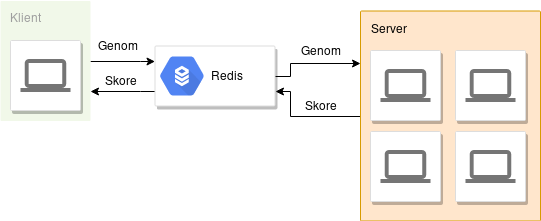
\includegraphics[scale=0.5]{distributed}
	\caption[Schéma distribuovaných výpočtů]{Schéma distribuovaných výpočtů}
	\label{fig:distributed}
\end{figure}

Tento přístup má několik výhod a to:

\begin{enumerate}
	\item Robustnost - Pokud jeden nebo více zpracovatelů selže (je například odpojen ze sítě) je možné pokračovat ve vyhodnocování (neúspěšný úkol lze vrátit zpátky do fronty). Toto v kombinaci s výše zmíněným docker swarmem znamená, že jakýkoliv výpočetní uzel lze kdykoliv vypnout a po znovu zapojení do sítě si načte nejnovější konfiguraci a začne znovu vyhodnocovat bez potřeby jakékoliv manipulace s jakoukoliv částí swarmu.
	\item Dobré rozložení zátěže - Jelikož si zpracovatel vytahuje úkoly z~fronty, je vždy optimálně zatížen, a není třeba řešit rozložení mezi různě výkonnými a zatíženými počítači.
	\item Škálovatelnost - problém lze škálovat až do doby, kdy počet procesorů nepřesáhne počet potřebných simulací. Chceme-li tedy vypočítat generaci o tisíci jedincích můžeme na ně nasadit až tisíc procesorů.
\end{enumerate}

Lze i namítnout, že se zde projevuje určitá režie při síťové komunikaci se serverem, což může být zdrojem určitého zpomalení. Nicméně se toto zpomalení neprojevilo v~průběhu testování clusteru. Právě naopak bylo naměřeno 10 násobné zrychlení oproti výpočtu na jednom počítači.

\kapitola{Klientská část}
Klientská část byla navržena tak, aby byla schopná vizualizovat průběh algoritmu NEAT a zároveň měla možnost znovu vyhodnocení existujících genomů vygenerovaných serverovou částí. První požadavek vznikl na základě konzultace s vedoucím, který chtěl algoritmus neurovoluce demonstrovat v hodinách předmětu VUI2. Druhý požadavek vznikl z důvodu potřeby vizualizace řešení, které generoval sever.

\sekce{Vizualizace}
Vizualizace se skládá z jednoduchého rozhraní, které lze vidět na obrázku \ref{fig:visualization}. V horní části je graf, zobrazující průběh genetického algoritmu. Lze v něm nalézt fitness nejlepšího, nejhoršího a průměrného jedince v populaci.

Další část se skládá z konfigurovatelného množství simulačních prostředí. Jednotliví jedinci v generaci jsou pak rovnoměrně rozloženi mezi všechna simulační prostředí a uživatel může pozorovat vývoj jedinců v realném čase.

Poslední tlačítko slouží k urychlení simulace. Způsobí to, že se simulace začne obnovovat bez vykreslování. Toto jí značně zrychlí.

\begin{figure}[h!]
	\centering
	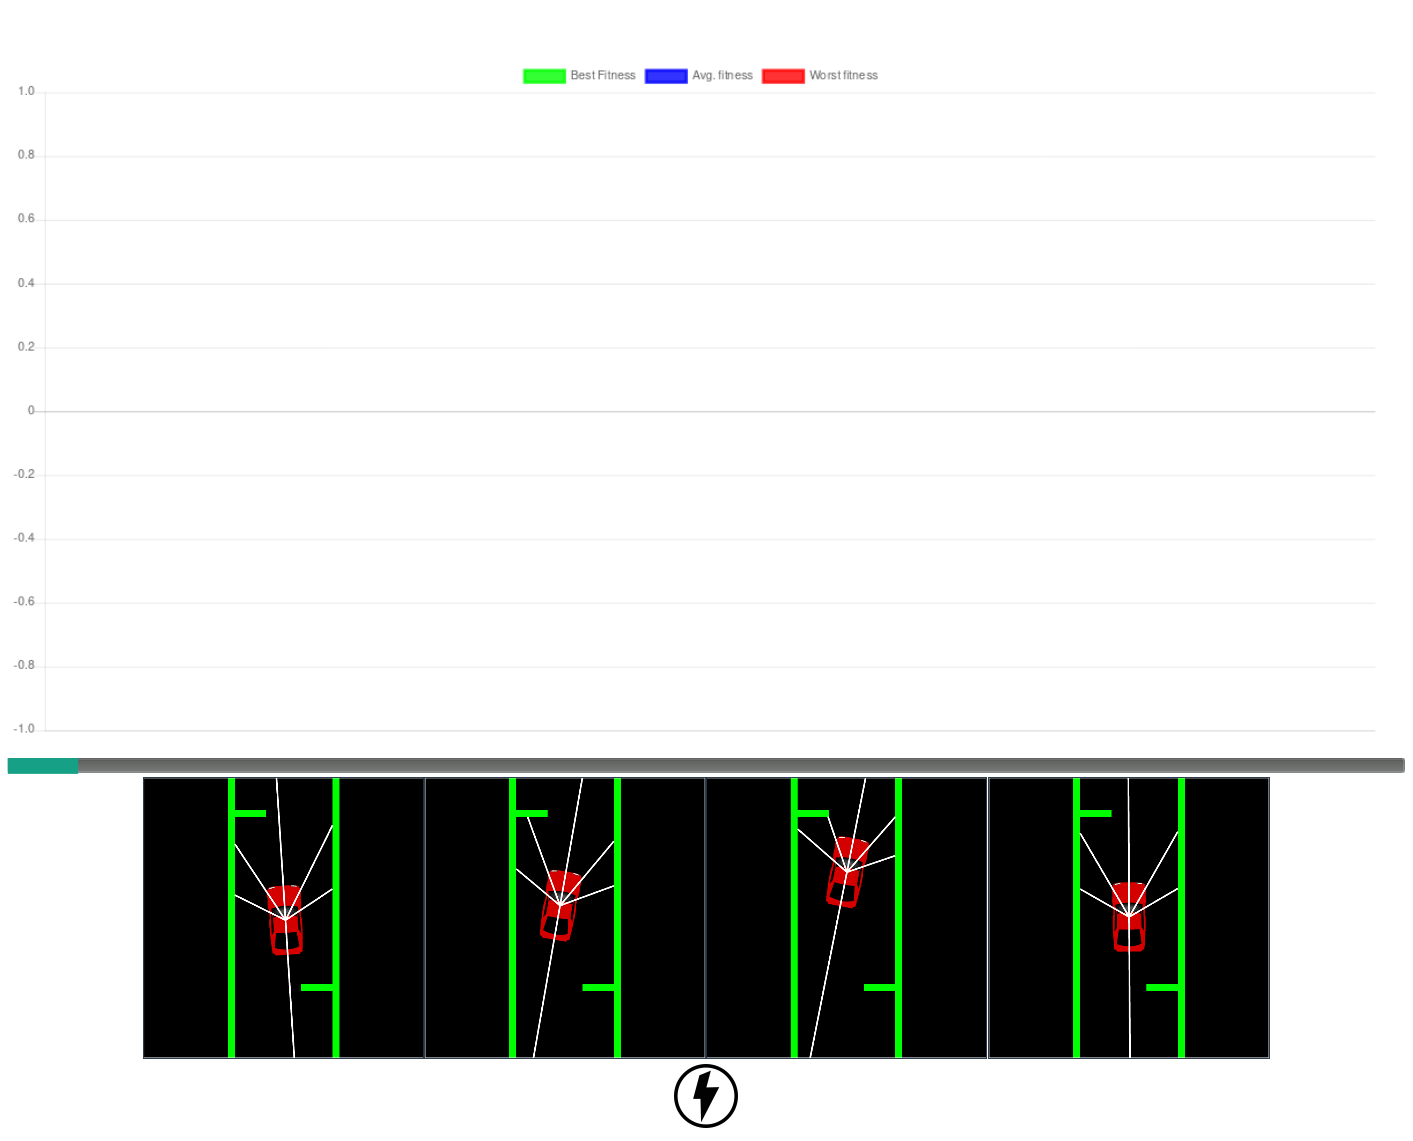
\includegraphics[width=0.6\linewidth]{visualization}
	\caption{Uživatelské rozhraní klientské části}
	\label{fig:visualization}
\end{figure}


\kapitola{Experimenty}
Po návrhu simulačního prostředí byl agent vyzkoušen v~několika situacích se stupňující se obtížností. Každá simulace probíhala s~1000 jedinci po 2000 generací. Ačkoliv je pravděpodobné, že by delší doba evaluace by pravděpodobně vyústila v lepší výsledky její výpočet v různých konfiguracích se ukázal jako příliš časově náročný navíc empirické pozorování ukázalo, že tato konfigurace poskytuje dostatečně dobré výsledky za snesitelný čas. 

S ohledem na časovou náročnost výpočtů (výpočet tisíce generací trvá na výpočetním clusteru přibližně 5 hodin) byly zkoumany jen tyto konfigurace:
\sekce{Nekonečná silnice ve tvaru I}
Agent byl umístěn do nekonečné rovné silnice ve tvaru I. Cílem bylo pozorovat, zda se agent bude schopný naučit řídit rovně. Agent po tisící generací dosáhl fitness 3 500 a naučil úspěšně kývavým pohybem udržet uprostřed vozovky.
\begin{figure}[h]
	\centering
	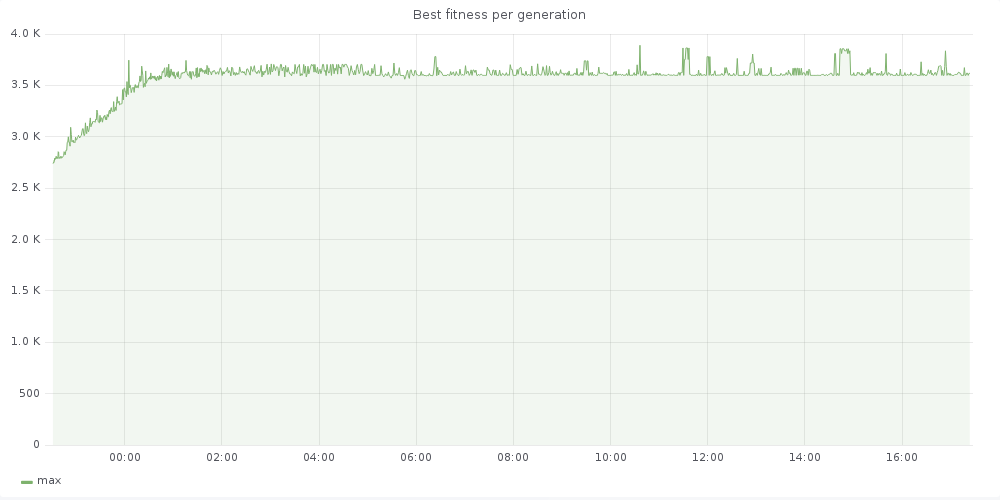
\includegraphics[scale=0.4]{I_fitness}
	\caption{Fitness agenta v průběhu času}
	\label{fig:i-experiment}
\end{figure}

\kapitola{Možná vylepšení}
Tato kapitola se bude zabývat možnými vylepšení současného řešení.
\kapitola{Závěr} 

%\input{zaverprace.tex}
\begin{literatura}
	\citace{practitionersApproach}{BUDUMA, Nikhil 2017}{
		\autor{BUDUMA, Nikhil.} \nazev{Fundamentals of deep learning: designing next-generation machine intelligence algorithms.} Sebastopol: O'Reilly, 2017. ISBN 978-149-1925-614.}
	\citace{fundementalsOfDeepLearning}{PATTERSON, Josh. 2017}{\autor{PATTERSON, Josh.} \nazev{Deep learning : a practitioner's approach}
		\nazev{Deep learning : a practitioner's approach. 1.} Beijing ; Boston ; Farnham ; Sebastopol ; Tokyo: O'Reilly, 2017. ISBN 978-1-491-91425-0.}
	\citace{geneticAlgorithms}{MITCHELL, Melanie., 1996}{\autor{MITCHELL, Melanie.} \nazev{An introduction to genetic algorithms.} Cambridge: Bradford Book, c1996. ISBN 0-262-13316-4.}
\end{literatura}

\prilohy{}
\priloha{CD se zdrojovým kódem}
\priloha{Tabulka s naměřenými rychlostmi clusteru}

\begin{table}[H]
	\begin{tabular}{lccccc}
		Jedinců & Cluster & Cluster-2 & Cluster-3 & Cluster-4 & Phenom II X4 965 \\
		100     & 9.853   & 6.1684    & 3.6887    & 3.7583    & 6.5186           \\
		200     & 13.3993 & 9.126     & 6.451     & 7.1599    & 10.9839          \\
		300     & 15.5628 & 10.5351   & 9.08      & 10.8206   & 16.8723          \\
		400     & 17.7699 & 13.6263   & 11.9285   & 13.0231   & 23.5019          \\
		500     & 19.1542 & 14.303    & 15.349    & 16.3707   & 31.7831          \\
		600     & 20.4675 & 18.8677   & 18.571    & 20.0113   & 37.3242          \\
		700     & 23.4671 & 20.1617   & 20.9039   & 23.7305   & 40.66            \\
		800     & 25.07   & 23.3143   & 24.9978   & 26.3178   & 44.8019          \\
		900     & 29.3611 & 28.1234   & 26.6288   & 29.6816   & 52.8829          \\
		1000    & 30.5498 & 28.7635   & 29.5586   & 33.5195   & 62.8967          \\
		1100    & 32.2825 & 32.0137   & 30.7372   & 37.2753   & 65.2363          \\
		1200    & 34.3818 & 31.8152   & 34.0371   & 42.1325   & 72.2926          \\
		1300    & 37.3422 & 35.8219   & 37.4416   & 40.3347   & 75.2937          \\
		1400    & 38.4452 & 41.3896   & 38.6274   & 41.3493   & 81.1193          \\
		1500    & 40.0487 & 43.225    & 43.4606   & 43.9233   & 81.3101         
	\end{tabular}
	\label{tbl:benchmark}
\end{table}

\end{document}

